\chapter{SPICE}

SPICE is an acronym (come on this is engineering of course it is an cutsie acronym to try to make it memorable) that stands for Simulation Program with Integrated Circuit Emphasis.  SPICE is often used as a simulator for circuit layout, and is thus usually incorporated into EDA (Electronic Design Analysis tools) like OrCAD or Mentor Graphics.  I will cover a separate SPICE tool called 5SPICE, which was designed for prototyping, and is free for educational use.

SPICE allows us to simulate a circuit without having to build it.  You can select actual component families, operating temperatures, and other operating conditions.  This allows a more accurate simulation, and thus less prototyping is needed.  This saves a lot of time and money, while improving the quality of the design, by allowing design changes in the simulation.

\raggedbottom\pagebreak
We will create an inverter gate using a transistor and some resistors.  First we need to put a transistor in our blank schematic.  We do this by selecting the NPN transistor symbol (if you don't know it, the name will appear in the tool tip when you hover) off the diode button on the right button bar.  When we have placed it by left clicking, we right click twice (once to end adding transistors and the second to edit the transistor we place).  A dialog will appear, from which you should select ``BC848C'' then click ``ok'' to accept.  Your screen should look like below.

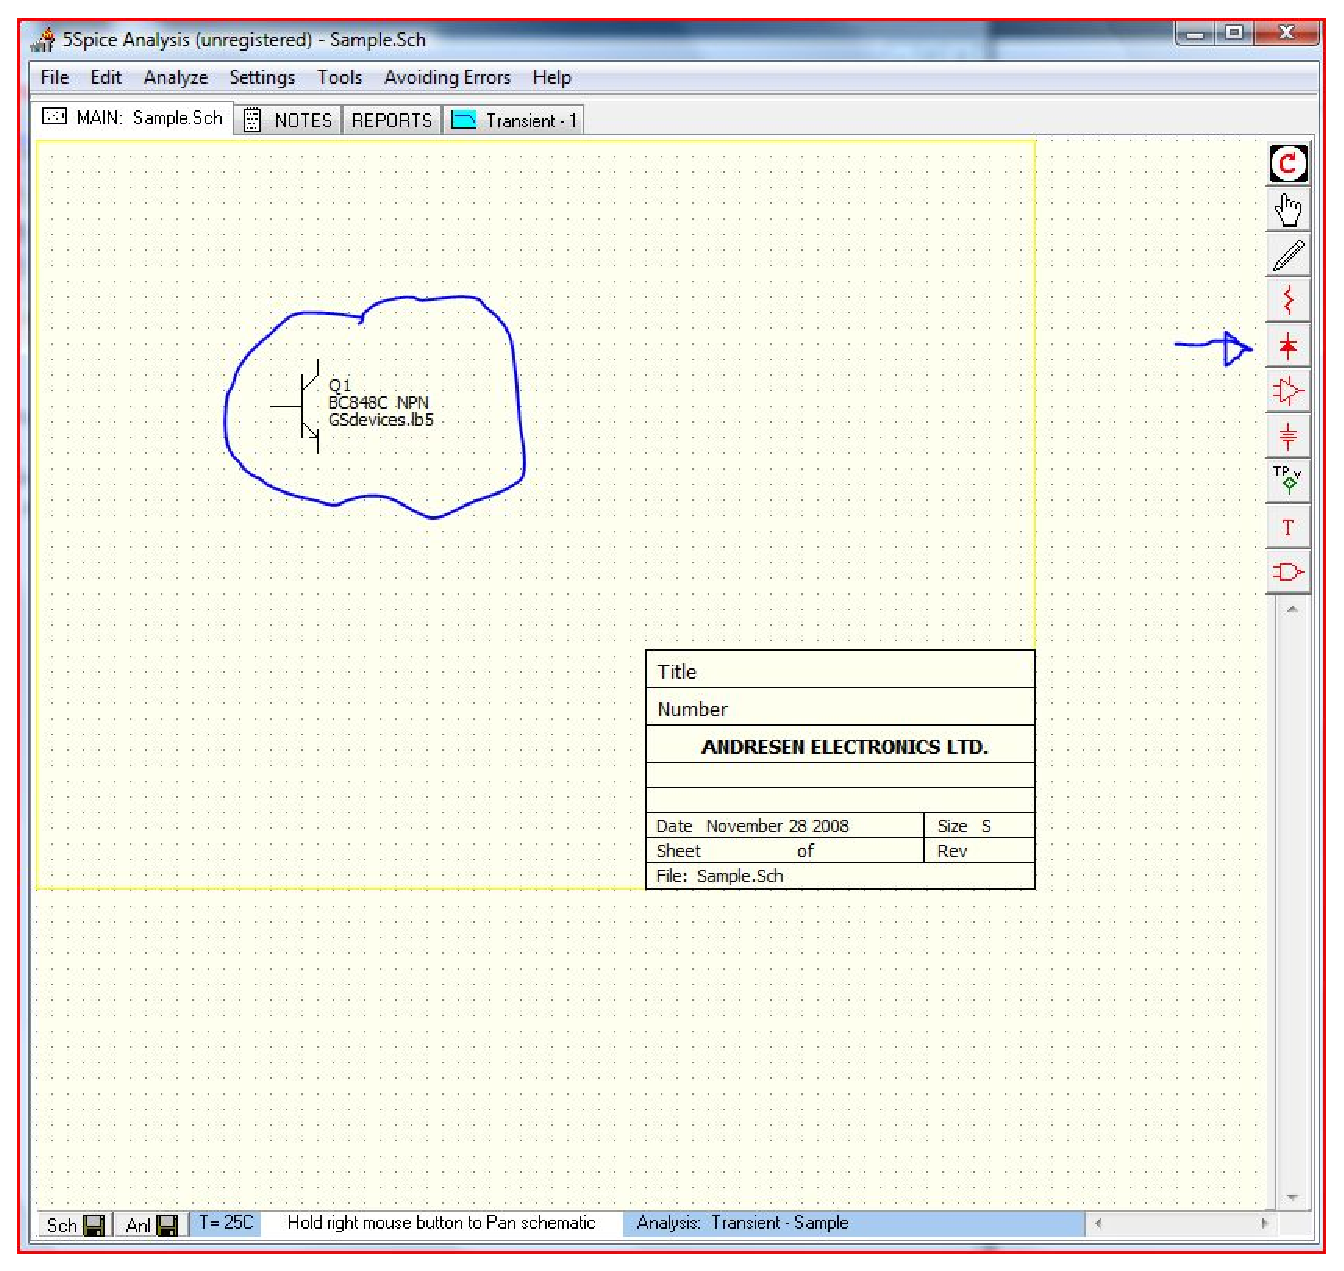
\includegraphics[width=\textwidth]{graphics/5spiceTransistora.eps}

\raggedbottom\pagebreak
We now need to add two resistors to keep the current flows within reason.  Resistors are selected from the resistor button on the right button bar.  Place two resistors on the sheet.  Right click to end adding and then right click one to edit.  Change the resistance to 100 (ohms is implicit) then click ok.  Move this one to the collector, to keep the current from collector to emitter to a reasonable value.  Now edit the other so it is also 100 ohms and click ok.  Right click it again and rotate.  Drag to the gate.  You schematic should look as follows.

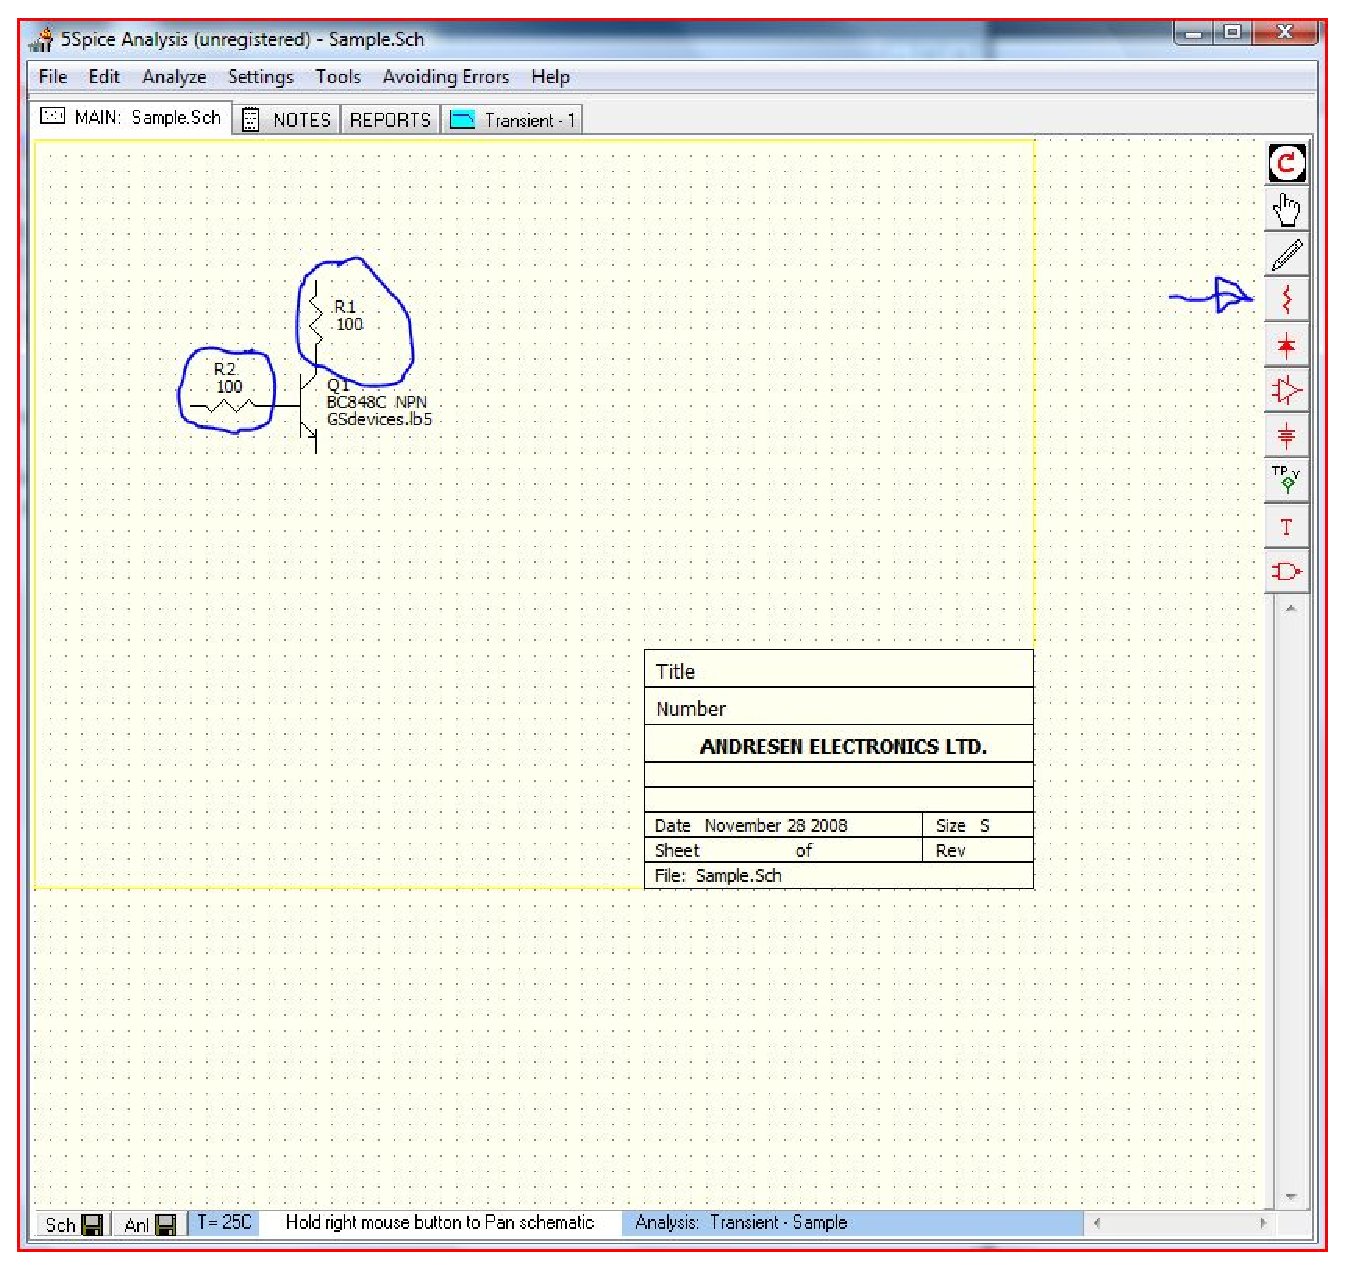
\includegraphics[width=\textwidth]{graphics/5spiceResistora.eps}

\raggedbottom\pagebreak
We know need to add several items from the power source button.  Start with a DC source to supply power to the transistor.  We will need to edit it so it has 5 volts.  Since we don't want to drag wires all over the schematic (we could, I just think it looks ugly) we will use two voltage points to connect the DC source to the resistor on the source.  Let's edit them to name it VpVCC.  Now add an AC voltage source.  When you edit its properties there will be several tabs so select the one called transient.  Select square wave, 5 volts peak to peak, 2.5 volts bias (so it goes 0-5 not -2.5 to 2.5), a frequency of 1, and a rise time of .1.  I also set the delay to 1 so it stays at 0 volts for a second before transitioning.  We will again add two voltage points to keep things neat, this time putting them on the input signal and calling them VpSignal.  Now add three grounds where marked on the diagram.

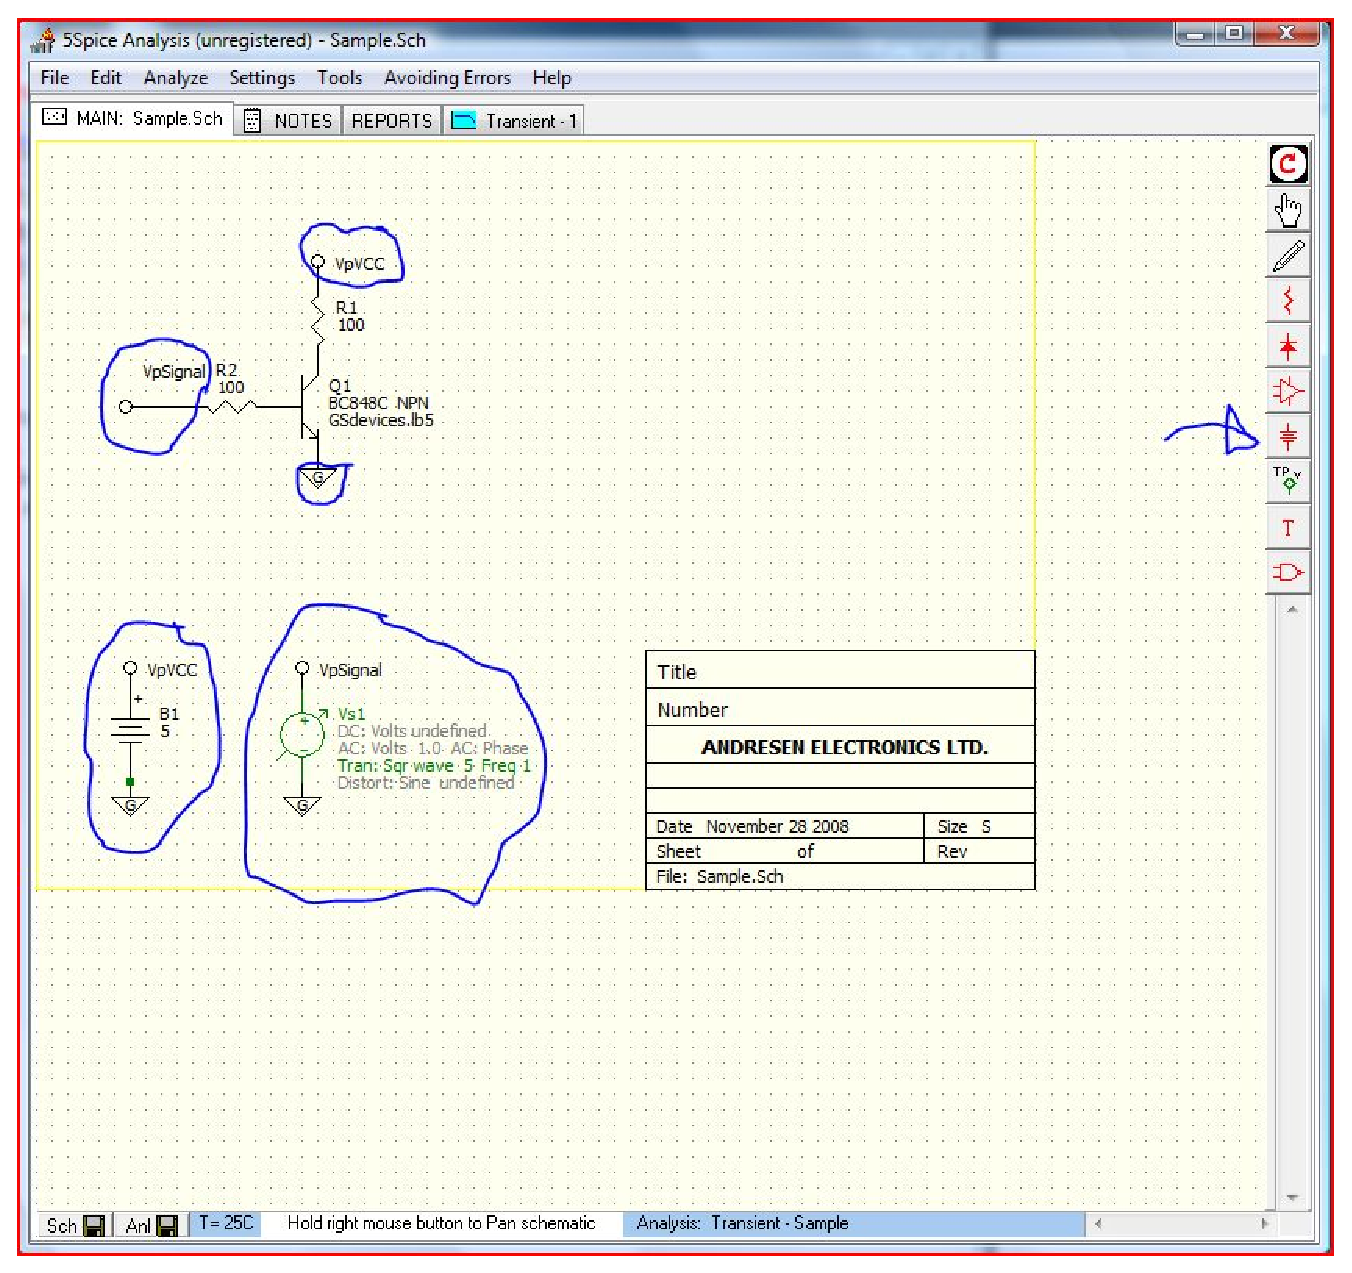
\includegraphics[width=\textwidth]{graphics/5spiceVoltsa.eps}

\raggedbottom\pagebreak
Now we need to add two test points, so we graph something.  You can only plot from test points.  To keep it neat I used wires to connect them.

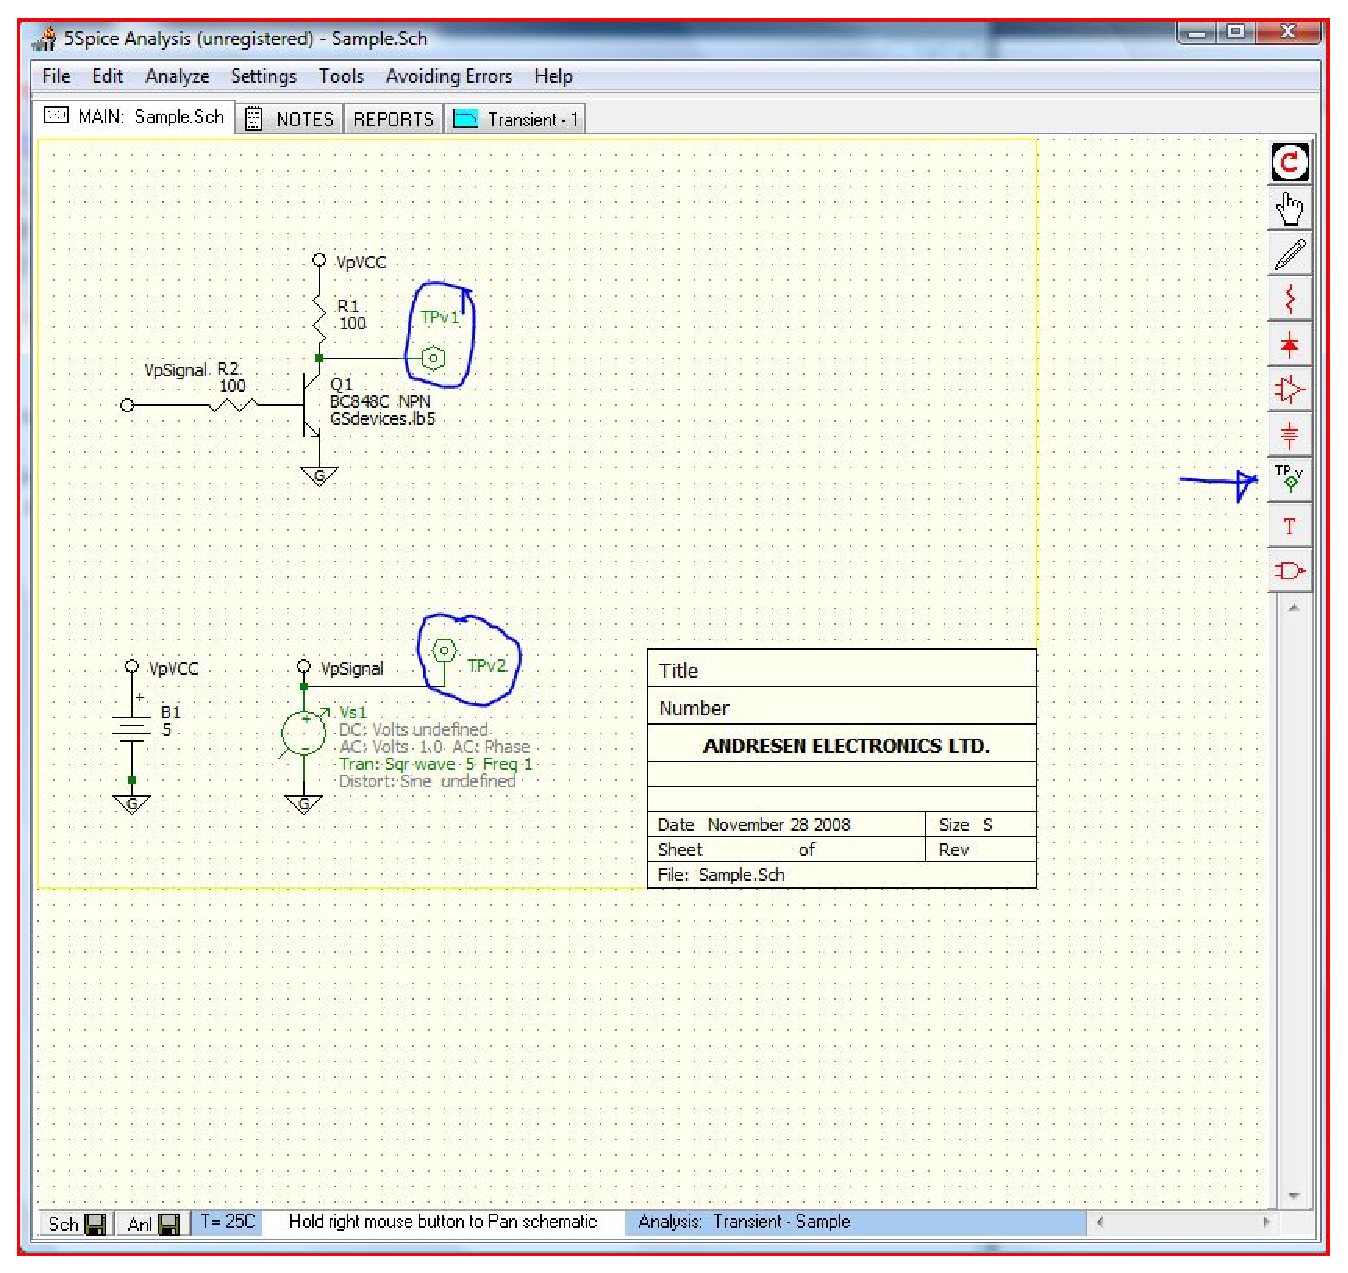
\includegraphics[width=\textwidth]{graphics/5spiceTPa.eps}

\raggedbottom\pagebreak
We now need to set the defaults for the simulator.  From the Analyze menu, select ``Project Defaults\dots'' then select the Analysis tab.  Pick transient analysis using Vs1 and simulate from 0 to 10 seconds.

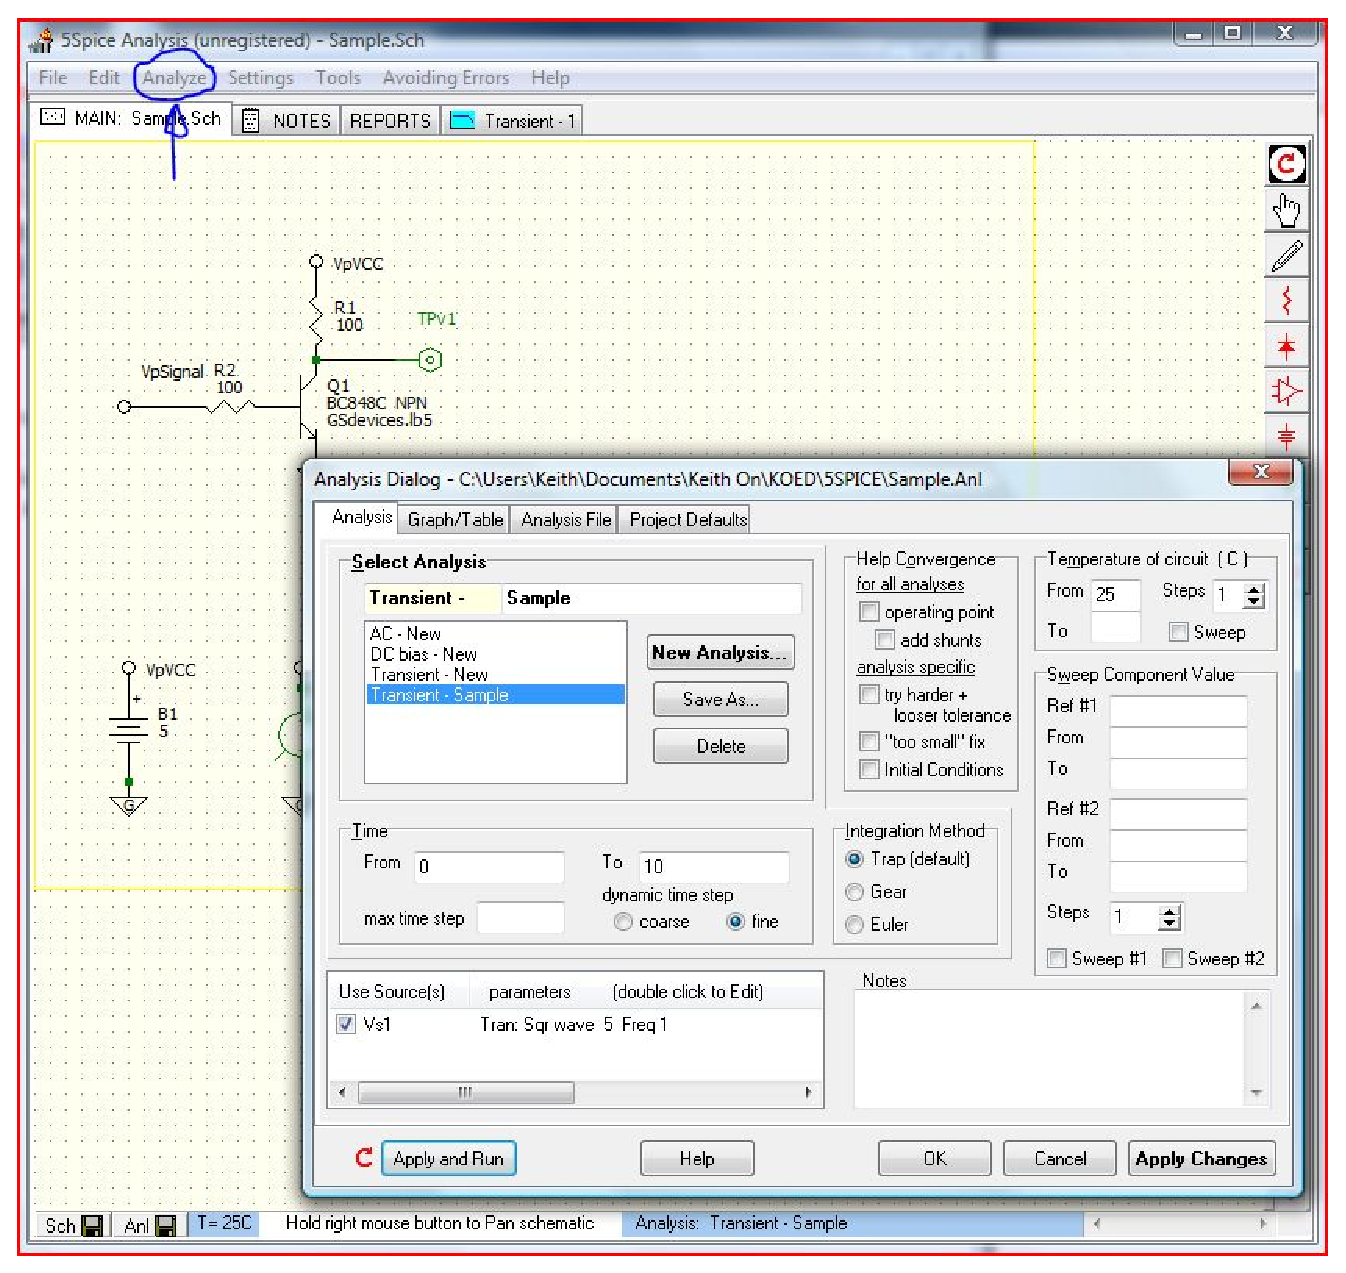
\includegraphics[width=\textwidth]{graphics/5spiceDefaultsa.eps}

\raggedbottom\pagebreak
Now select the Graph/Table tab and under Plots, select TPv1 with Left axis and TPv2 with Left axis.  Note if you don't select the axis it is off by default.  Then set the vertical axis to go from -1 to 6 so there is some room around the graph (again for aesthetics).  Save and Run.

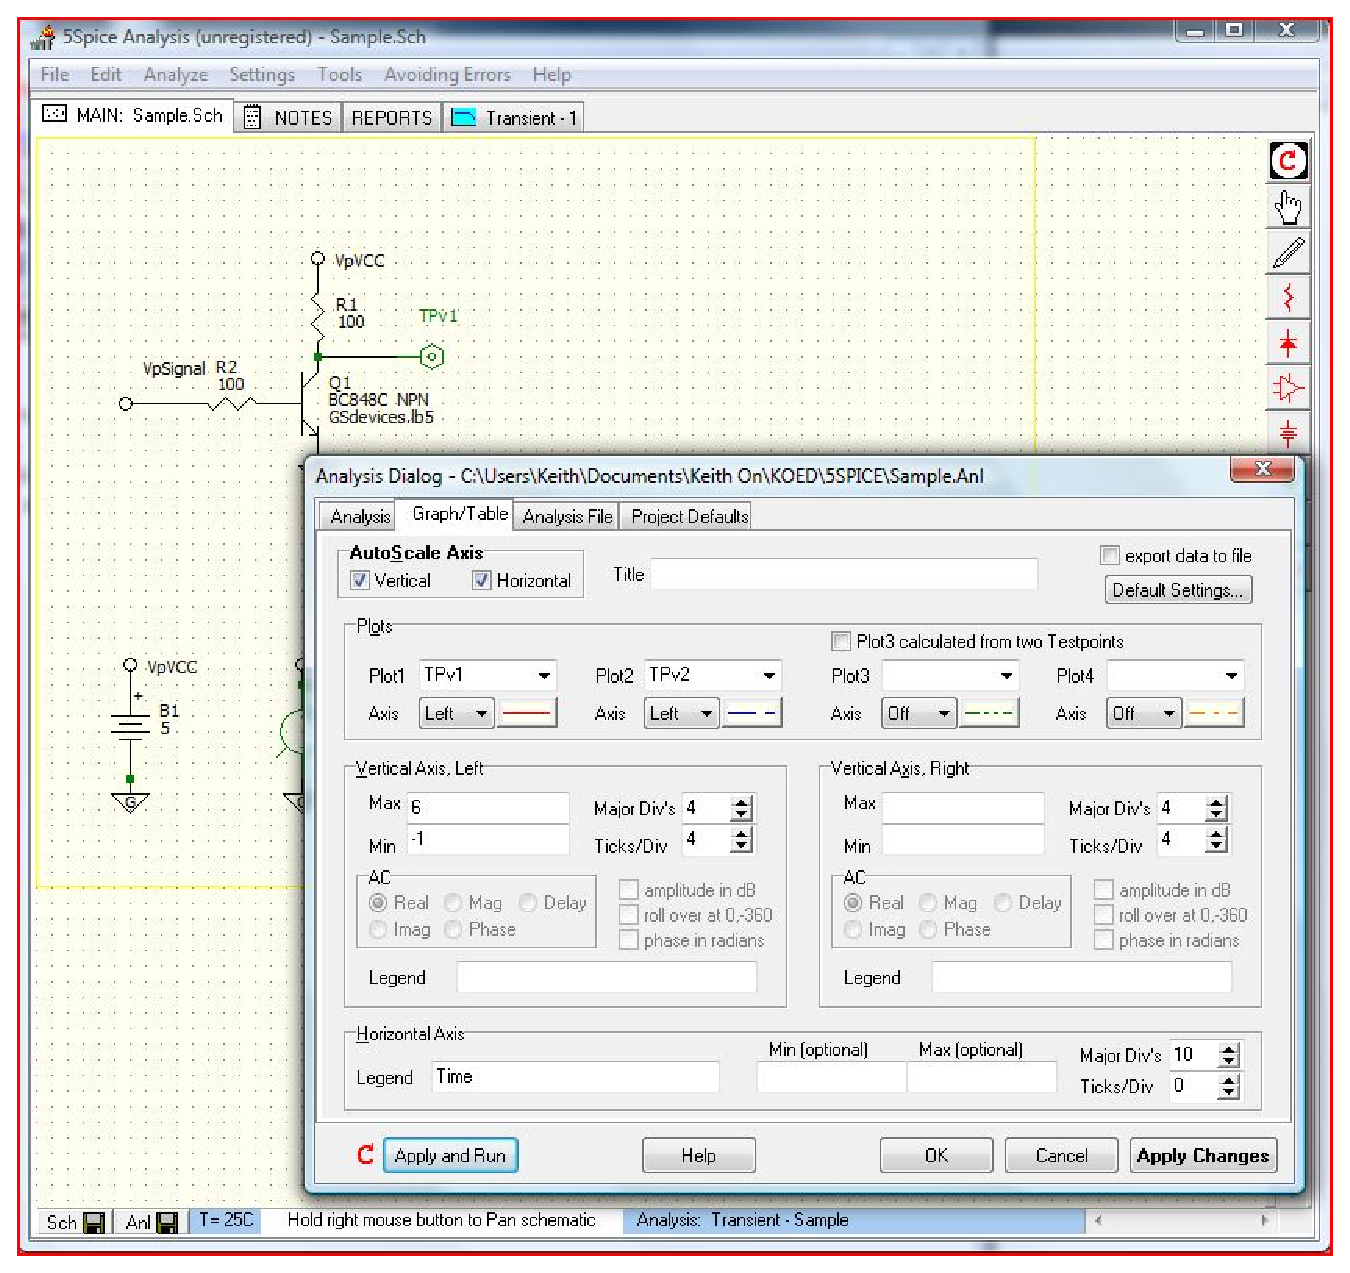
\includegraphics[width=\textwidth]{graphics/5spiceGraph.eps}

\raggedbottom\pagebreak
You will get a graph like below after a few seconds.  Note the graph shows we have an inverter.  You will also note the inverted signal does not go to zero exactly due to the resistors.  If you play with the resistances you will get some interesting results.  Try and see.  You should also see the cyan circle with the vertical line at the top of the graph.  It is the measurement device, and it is the selector for the x,y data on the top right.  Try moving it and reading the voltages.

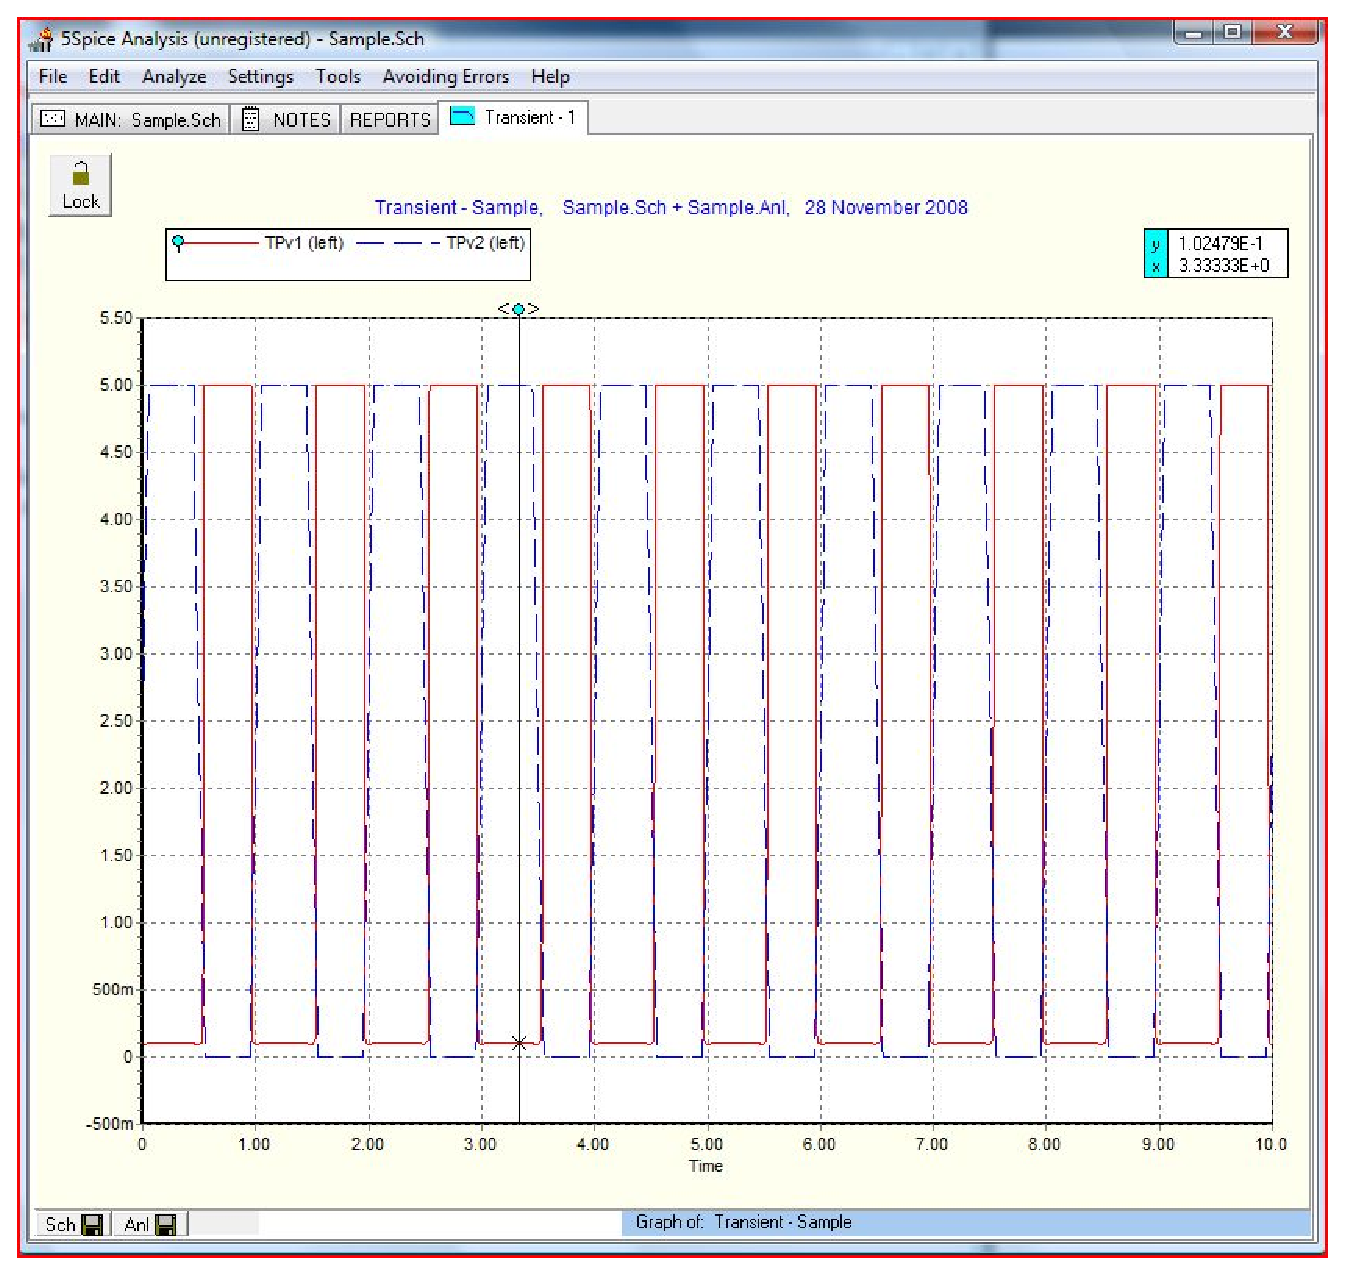
\includegraphics[width=\textwidth]{graphics/5spiceOut.eps}
